
\documentclass[
a4paper,     %% defines the paper size: a4paper (default), a5paper, letterpaper, ...
% landscape,   %% sets the orientation to landscape
% twoside,     %% changes to a two-page-layout (alternatively: oneside)
% twocolumn,   %% changes to a two-column-layout
 headsepline, %% add a horizontal line below the column title
footsepline, %% add a horizontal line above the page footer
titlepage,   %% only the titlepage (using titlepage-environment) appears on the first page (alternatively: notitlepage)
 halfparskip,     %% insert an empty line between two paragraphs (alternatively: halfparskip, ...)
% leqno,       %% equation numbers left (instead of right)
 fleqn,       %% equation left-justified (instead of centered)
% tablecaptionabove, %% captions of tables are above the tables (alternatively: tablecaptionbelow)
% draft,       %% produce only a draft version (mark lines that need manual edition and don't show graphics)
% 10pt         %% set default font size to 10 point
% 11pt         %% set default font size to 11 point
12pt         %% set default font size to 12 point
]{scrartcl}  %% article, see KOMA documentation (scrguide.dvi)



%%%%%%%%%%%%%%%%%%%%%%%%%%%%%%%%%%%%%%%%%%%%%%%%%%%%%%%%%%%%%%%%%%%%%%%%%%%%%%%%
%%%
%%% packages
%%%

%%%
%%% encoding and language set
%%%

%%% ngerman: language set to new-german
\usepackage{ngerman}

%%% babel: language set (can cause some conflicts with package ngerman)
%%%        use it only for multi-language documents or non-german ones
%\usepackage[ngerman]{babel}

%%% inputenc: coding of german special characters
\usepackage[utf8]{inputenc}

%%% fontenc, ae, aecompl: coding of characters in PDF documents
\usepackage[T1]{fontenc}
\usepackage{ae,aecompl}

%%%
%%% technical packages
%%%

%%% amsmath, amssymb, amstext: support for mathematics
\usepackage{amsmath,amssymb,amstext}

%%% psfrag: replace PostScript fonts
%\usepackage{psfrag}

%%% listings: include programming code
%\usepackage{listings}

%%% units: technical units
\usepackage{units}

%%%
%%% layout
%%%

%%% scrpage2: KOMA heading and footer
%%% Note: if you don't use this package, please remove 
%%%       \pagestyle{scrheadings} and corresponding settings
%%%       below too.
\usepackage{scrpage2}

%%%
%%% PDF
%%%

\newif\ifpdf
  \ifx\pdfoutput\undefined
     \pdffalse
  \else
     \pdfoutput=1
     \pdftrue
  \fi

%%% Should be LAST usepackage-call!
%%% For docu on that, see reference on package ``hyperref''
\ifpdfoutput{%   (definitions for using pdflatex instead of latex)

  %%% graphicx: support for graphics
  \usepackage[pdftex]{graphicx}

  \pdfcompresslevel=9

  %%% hyperref (hyperlinks in PDF): for more options or more detailed
  %%%          explanations, see the documentation of the hyperref-package
  \usepackage[%
    %%% general options
    pdftex=true,      %% sets up hyperref for use with the pdftex program
    %plainpages=false, %% set it to false, if pdflatex complains: ``destination with same identifier already exists''
    %
    %%% extension options
    backref=true,      %% if true, adds a backlink text to the end of each item in the bibliography
    pagebackref=false, %% if true, creates backward references as a list of page numbers in the bibliography
    colorlinks=false,   %% turn on colored links (true is better for on-screen reading, false is better for printout versions)
    %
    %%% PDF-specific display options
    bookmarks=true,          %% if true, generate PDF bookmarks (requires two passes of pdflatex)
    bookmarksopen=false,     %% if true, show all PDF bookmarks expanded
    bookmarksnumbered=false, %% if true, add the section numbers to the bookmarks
    %pdfstartpage={1},        %% determines, on which page the PDF file is opened
    pdfpagemode=None         %% None, UseOutlines (=show bookmarks), UseThumbs (show thumbnails), FullScreen
  ]{hyperref}


  %%% provide all graphics (also) in this format, so you don't have
  %%% to add the file extensions to the \includegraphics-command
  %%% and/or you don't have to distinguish between generating
  %%% dvi/ps (through latex) and pdf (through pdflatex)
  \DeclareGraphicsExtensions{.pdf}

}{%else   (definitions for using latex instead of pdflatex)

  \usepackage[dvips]{graphicx}

  \DeclareGraphicsExtensions{.eps}

  \usepackage[%
    dvips,           %% sets up hyperref for use with the dvips driver
    colorlinks=false %% better for printout version; almost every hyperref-extension is eliminated by using dvips
  ]{hyperref}

}


%%% sets the PDF-Informations options
%%% (see fields in Acrobat Reader: ``File -> Document properties -> Summary'')
%%% Note: this method is better than as options of the hyperref-package (options are expanded correctly)
\hypersetup{
  pdftitle={Einrichtung einer internen Firewall von Firma-a und Firma-b und LAN-to-LAN-VPN Firma-a	(Server)	
nach	 Firma-b(Client)}, %%
  pdfauthor={}, %%
  pdfsubject={IT Sicherheitsarchitekturen}, %%
  pdfcreator={Accomplished with LaTeX2e and pdfLaTeX with hyperref-package.}, %% 
  pdfproducer={}, %%
  pdfkeywords={} %%
}


%%%%%%%%%%%%%%%%%%%%%%%%%%%%%%%%%%%%%%%%%%%%%%%%%%%%%%%%%%%%%%%%%%%%%%%%%%%%%%%%
%%%
%%% user defined commands
%%%

%%% \mygraphics{}{}{}
%% usage:   \mygraphics{width}{filename_without_extension}{caption}
%% example: \mygraphics{0.7\textwidth}{rolling_grandma}{This is my grandmother on inlinescates}
%% requires: package graphicx
%% provides: including centered pictures/graphics with a boldfaced caption below
%% 
\newcommand{\mygraphics}[3]{
  \begin{center}
    \includegraphics[width=#1, keepaspectratio=true]{#2} \\
    \textbf{#3}
  \end{center}
}

%%%%%%%%%%%%%%%%%%%%%%%%%%%%%%%%%%%%%%%%%%%%%%%%%%%%%%%%%%%%%%%%%%%%%%%%%%%%%%%%
%%%
%%% define the titlepage
%%%

 \subject{IT Sicherachitekturen}   %% subject which appears above titlehead
% \titlehead{} %% special heading for the titlepage

%%% title
\title{Einrichtung einer internen Firewall von Firma-a und Firma-b, sowie LAN-to-LAN-VPN von Firma-a (Server)	
nach	 Firma-b(Client)}

%%% author(s)
\author{Paul Drautzburg \and
Georg Mohr}

%%% date
\date{HTWG Konstanz, Sommersemester 2018}

% \publishers{}

% \thanks{} %% use it instead of footnotes (only on titlepage)

% \dedication{} %% generates a dedication-page after titlepage


%%% uncomment following lines, if you want to:
%%% reuse the maketitle-entries for hyperref-setup
%\newcommand\org@maketitle{}
%\let\org@maketitle\maketitle
%\def\maketitle{%
%  \hypersetup{
%    pdftitle={\@title},
%    pdfauthor={\@author}
%    pdfsubject={\@subject}
%  }%
%  \org@maketitle
%}


%%%%%%%%%%%%%%%%%%%%%%%%%%%%%%%%%%%%%%%%%%%%%%%%%%%%%%%%%%%%%%%%%%%%%%%%%%%%%%%%
%%%
%%% set heading and footer
%%%

%%% scrheadings default: 
%%%      footer - middle: page number
\pagestyle{scrheadings}

%%% user specific
%%% usage:
%%% \position[heading/footer for the titlepage]{heading/footer for the rest of the document}

%%% heading - left
% \ihead[]{}

%%% heading - center
% \chead[]{}

%%% heading - right
 %\ohead[]{}

%%% footer - left
% \ifoot[]{}

%%% footer - center
% \cfoot[]{}

%%% footer - right
% \ofoot[]{}



%%%%%%%%%%%%%%%%%%%%%%%%%%%%%%%%%%%%%%%%%%%%%%%%%%%%%%%%%%%%%%%%%%%%%%%%%%%%%%%%
%%%
%%% begin document
%%%

\begin{document}

 \pagenumbering{roman} %% small roman page numbers

%%% include the title
% \thispagestyle{empty}  %% no header/footer (only) on this page
 \maketitle

%%% start a new page and display the table of contents
 \newpage
 \tableofcontents

%%% start a new page and display the list of figures
 \newpage
 \listoffigures

%%% start a new page and display the list of tables
\newpage
 \listoftables

%%% display the main document on a new page 
 \newpage

 \pagenumbering{arabic} %% normal page numbers (include it, if roman was used above)

%%%%%%%%%%%%%%%%%%%%%%%%%%%%%%%%%%%%%%%%%%%%%%%%%%%%%%%%%%%%%%%%%%%%%%%%%%%%%%%%
%%%
%%% begin main document
%%% structure: \section \subsection \subsubsection \paragraph \subparagraph
%%%

\section{Motivation}
Im Zeitalter der Digitalisierung steigt der Grad der Vernetzung immer weiter an. Unternehmen, welche ihre Standorte über die ganze Welt verteilt haben, wollen Wege und Möglichkeiten haben ihre Arbeit sicher und Problemlos zu verrichten. Dafür ist es unerlässlich, dass verschiedene Standorte auf Ressourcen des anderen zugreifen können. Für solche Szenarien gibt es in der Netzwerktechnik und Netzwerkarchitektur verschiedene Lösungsansätze. 
Jedoch darf dabei ein wichtiger Aspekt nicht vernachlässigt werden, denn jedes Unternehmen hat Betriebsmittel und Informationen, welche es nicht Gefahren von außen aussetzten will. An diesem Punkt kommt der Begriff IT-Sicherheit ins Spiel und genau dieses Umfeld um den Begriff „IT-Sicherheit“ wird im Rahmen des Praktikums zur Lehrveranstaltung „IT-Sicherheitsarchitekturen“ untersucht. 
In den folgenden Kapiteln wird eine Problemstellung unter Laborbedingungen skizziert, welche ein Szenario wiederspiegelt, mit dem sich Unternehmen täglich konfrontiert sehen. Anschließend wird werden die Laborbedienungen und der Versuchsaufbau beschrieben. Aus der Problemstellung und dem Versuchsaufbau wird eine Lösung auf Grundlage, der damit zu Grunde liegenden Theorie, erarbeitet. Diese Lösung wird abschließend in die Laborumgebung implementiert und auf ihre Akzeptanz gegenüber der Problemstellung untersucht und in einem Fazit bewertet.   
\section{Problemstellung}
In diesem Kapitel wird die Laborumgebung eingeführt und beschrieben, sowie die damit verbundene Aufgaben-/Problemstellung skizziert.
\subsection{Laborumgebung und Versuchsaufbau}
\label{laborumgebung}
Im Labor wird die IT-Landschaft zweier Unternehmen „A“ und „B“ simuliert. Jedes Unternehmen besitzt ein lokales LAN, an denen die pot. Mitarbeiter angeschlossen sind, zudem gibt es mehrere Server mit Hilfe derer verschiedene Dienste angeboten werden sollen. 
Es folgt eine Liste an Diensten welche Angeboten werden sollen:
Internetzugang von den Mitarbeiter-Computern.
Zugang über HTTPS der Webseiten beider Unternehmen.
Eine Virtuelle Kopplung der beiden Unternehmen mit Hilfe einer sog. Site-to-Site Verbindung.
Jeder Mitarbeiter der Unternehmen soll die Möglichkeit haben, E-Mails über einen Mailsserver zu verschicken.  
Eine weitere wichtige Komponente in dieser IT-Landschaft sind die externen und internen Firewalls, da diese den Grundstein für eine sichere Umgebung legen. In dieser IT-Landschaft gibt es insgesamt 4 Firewalls, jedes Unternehmen hat jeweils eine interne und externe Firewall. Hinter den externen Firewalls beider Unternehmen liegt jeweils die sog. DMZ – Demilitarisierte Zone. In dieser Zone stehen üblicherweise die Unternehmensserver, diese werden nach außen hin von der externen Firewall und nach innen von der internen Firewall geschützt. Jede Firewall läuft auf einem Server, somit besteht die IT-Landschaft insgesamt aus 4 Servern auf welchen die Firewalls laufen, 2 Servern, welche die jeweiligen Unternehmensserver simulieren und einem Server welcher außerhalb der externen Firewall das Internet simulieren soll (vgl. Abb. \ref{fig:appStat}).

\begin{figure}[h]
	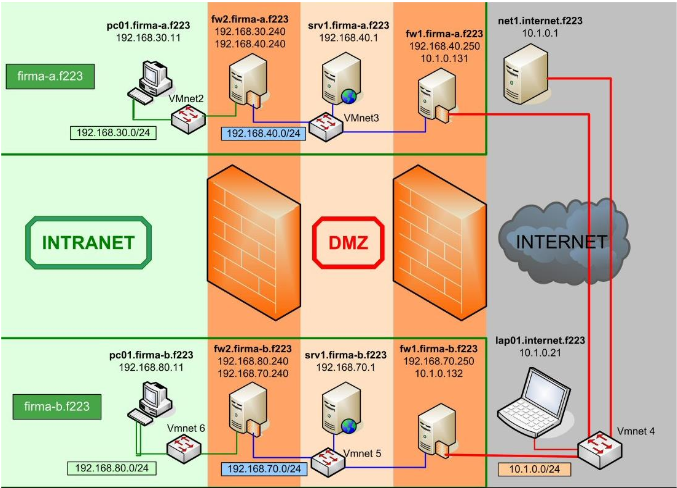
\includegraphics[width=\textwidth]{pictures/laborumgebung.png}
	\caption{Schematischer Aufbau der Laborumgebung im IT-Sicherheitslabor \cite{JueNeuSaDue}}
	\label{fig:appStat}
\end{figure}
Jede dieser angesprochenen Komponenten muss entsprechen konfiguriert werden, damit die angesprochenen Dienste fehlerfrei funktionieren können.
Technisch gesehen wird jeder dieser Server auf Grundlage einer virtuellen Maschine abgebildet.
Jede dieser Maschinen hat Linux als Betriebssystem installiert und vorkonfiguriert, jedoch ohne zusätzliche Pakte, nur die reine Grundinstallation   
Da die Implementierung und Installation aller dieser Dienste und der damit verbundenen Komponenten den Rahmen dieses Praktikums sprengen würde, werden die Aufgabenstellungen zuvor runtergebrochen. Die detaillierte Aufgabenstellung wird im nächsten Abschnitt eingeführt.

\subsection{Aufgabenstellung}
Wie schon im vorhergehenden Abschnitt beschrieben, gibt es mehrere Dienste, welche in der IT-Landschaft angeboten werden sollen. 
In diesem Bericht, wird die Virtuelle Kopplung der Unternehmen „A“ und „B“ durch eine „Site-to-Site-“ oder auch „LAN-to-LAN-“ genannt -Verbindung implementiert. 
Die Problemstellung gilt als gelöst, wenn es möglich ist, dass Unternehmen A eine gesicherte Verbindung zu Unternehmen B aufbauen kann und die jeweiligen internen Firewalls entsprechend konfiguriert sind. Die Konfiguration der externen Firewalls kann in dieser Aufgabe vernachlässigt werden, hierfür sollen die bereitgestellten internen Firewalls verwendet werden. 
//TODO Verweis auf Bilder, Begriffe zuordnen. 
 

\section{Theoretische Grundlagen}
In diesem Kapitel werden die theoretischen Grundlagen eingeführt, welche im Kontext der Aufgabestellung benötigt werden. Dies beschränkt sich auf drei Bereiche, die Netzwerkarchitekturen, Debian GNU Linux 7.11 und IP-Tables. Jede dieser genannten Bereiche wird innerhalb dieses Kapitels eingeführt und in den Aufgabenkontext eingeordnet. 
\subsection{Netzwerkarchitekturen}
Der Bereich Netzwerkarchitekturen ist ein sehr breites Gebiet, deshalb muss zuvor anhand der Anforderungen aus der Aufgabenstellung abgegrenzt werden.
Das Netzwerk des Labors besteht netzwerktechnisch grundlegend aus drei Bereichen dem Intranet, der Demilitarisierten Zone und dem Internet. 
Das Intranet zeichnet sich dadurch aus, dass es hinter einer internen Firewall liegt ... 

\subsection{Debian GNU Linux 7.11}
\subsection{IP-Tables}\label{iptables}
\subsection{OpenVPN}
\section{Lösungsskizze}
In diesem Kapitel wird sich mit dem Thema befasst, wie sich eine Side-to-Side VPN Verbindung, die die Firmen A und B wie in Kapitel \ref{laborumgebung} beschrieben verbindet.
Dazu waren zu Beginn mehrere Vorüberlegungen zu tätigen. Dies sind zum einen, wie wird das innere Netz der Firmen A und B geschützt, dann welcher VPN Dienst kann für diesen Zweck verwendet werden und welche weiteren Strategien braucht es bei der Umsetzung der Security Policies der Firmen. 
\subsection{Firewall}
Wenn eine Firewall aufgebaut werden soll, muss sich zu beginn überlegt werden, welche allgemeine Strategie mit der Firewall gefahren werden soll. Das heißt sollen alle Verbindungen Standardmäßig freigegeben werden und nur explizit nicht erlaubt Verbindungen geblockt werden (Default-Allow-Strategy), oder sollen alle Verbindungen blockiert werden und nur die die explizit erlaubt wurden, geöffnet werden (Default-Deny-Strategy). Im Standardfall wird in Unternehmen, die Strategie Default-Deny verwendet, weshalb sich auch im Versuchsaufbau diese Strategie gewählt wurde. Eine Firewall wird mit Hilfe des Userspace-Programmes IPTABLES (siehe Kapitel \ref{iptables}) unter Linux realisiert. 



\section{Auswertung(Georg)}
\section{Fazit}


%%%
%%% end main document
%%%
%%%%%%%%%%%%%%%%%%%%%%%%%%%%%%%%%%%%%%%%%%%%%%%%%%%%%%%%%%%%%%%%%%%%%%%%%%%%%%%%

 \appendix  %% include it, if something (bibliography, index, ...) follows below

%%%%%%%%%%%%%%%%%%%%%%%%%%%%%%%%%%%%%%%%%%%%%%%%%%%%%%%%%%%%%%%%%%%%%%%%%%%%%%%%
%%%
%%% bibliography
%%%
%%% available styles: abbrv, acm, alpha, apalike, ieeetr, plain, siam, unsrt
%%%
 \bibliographystyle{alphadin}

%%% name of the bibliography file
 \bibliography{bib/literatur.bib}

\end{document}
%%% }}}
%%% END OF FILE
%%%%%%%%%%%%%%%%%%%%%%%%%%%%%%%%%%%%%%%%%%%%%%%%%%%%%%%%%%%%%%%%%%%%%%%%%%%%%%%%
%% Local Variables:
%% mode: outline-minor
%% OPToutline-regexp: "%% .*"
%% OPTeval: (hide-body)
%% emerge-set-combine-versions-template: "%a\n%b\n"
%% End:
%% vim:foldmethod=marker
